\documentclass{article}
\usepackage{amsmath,amssymb,amsfonts,amsthm,hyperref,enumerate}
\usepackage{graphicx, array, tabu} %package to manage images
\graphicspath{ {images/} }
\setcounter{secnumdepth}{5}
\usepackage[english]{babel}
\usepackage[utf8]{inputenc}
\usepackage{hyperref}
\newtheorem*{theorem}{Theorem}

\title{Complex Homotopy}
\author{Samuel Doud}
\date{April 27, 2016}

\begin{document}

\maketitle

\section{Introduction}
    Complex Homotopy is a simple \textit{Python} application that maps complex numbers from to the complex plane to the complex plane. Formally,
    $$T:\mathbb{C}\Rightarrow \mathbb{C}.$$
    Throughout this documentation, I will refer to the complex numbers as $\mathbb{C}$. A complex number is a mixture of imaginary and real numbers. The imaginary number $i$ is equal to $\sqrt{-1}$. It can be helpful to imagine the complex numbers as a plane, much like the $xy-\text{plane}$, however, on the $xy-\text{plane}$ we are visualing a function. On the complex plane, we are simply visualizing a set. That is were the use of this program comes in.
    Observe the function 
    $$y=x^{2}$$
    Now, observe the same function on the complex "unit grid" and "unit circle".
    $$f(z) = z^{2}$$
    \begin{figure}[h]
        \centering
        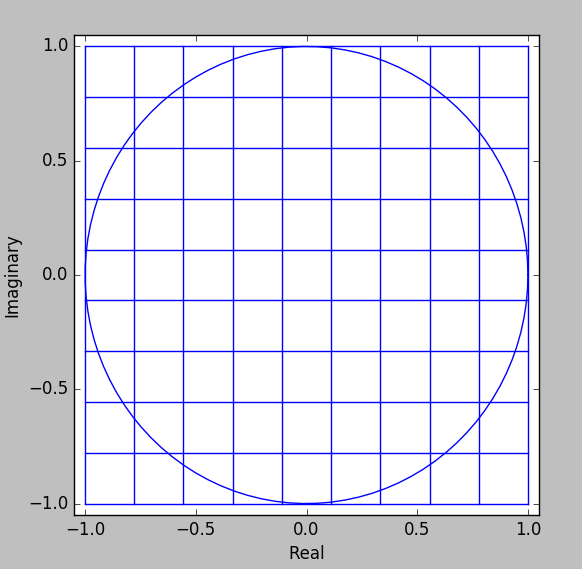
\includegraphics[scale=.5]{z}
        \caption{$z$}
        \label{fig:my_label}
    \end{figure}
    \begin{figure}[h]
        \centering
        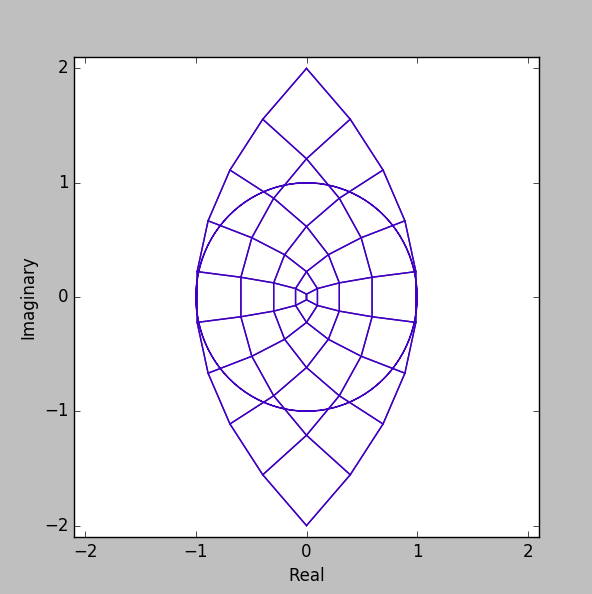
\includegraphics[scale=.5]{z2}
        \caption{$z^{2}$}
        \label{fig:my_label}
    \end{figure}
    \begin{figure}[h]
        \centering
        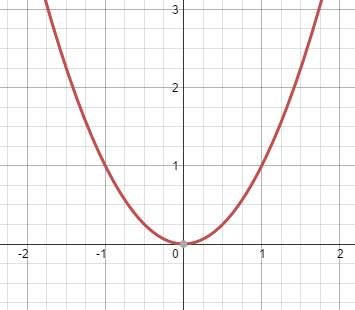
\includegraphics[scale=.66]{x2}
        \caption{$y=x^{2}$}
        \label{fig:my_label}
    \end{figure}
    Notice how two images were needed for the complex function. With the $xy$, we can intuitively see the result of the function from the graph, but the complex function is not so easy. In fact, squaring a complex number squares its absolute value and increases its angle measure two-fold. But how would you know that other than analyzing the function?\\
    This program animates the image of $z$ onto $f(z)$ so it is easier for students to observe what is actually occurring with the complex function. Hopefully, it can become as intuitive as any $xy$ function.
    a.  An Overview of your project
    b.  A description of your successes (i.e., what did you accomplish).
    c.  Obstacles and changes of directions (i.e., how did your project change form over the semester, based on what you experienced)
    d.  What did you learn?  
    e.  Future directions (i.e., if you had one more month?).
\section{Successes}
    The initial goal of this project was to create a system in which a user could watch a set of points be operated on by a complex function over time. In that sense, this project was highly successful. This system is in place and mostly works. There are some features that you would see on a graphing calculator that are not yet implemented, but they are in the pipeline and more importantly, they are secondary to the actual graphing.
\section{Obstacles and changes}
    \begin{itemize}
        \item Caching lines. The most difficult computation is not projecting the points, its calculating the arrangement of the lines and creating the line objects themselves.
        \item Eval exposure. I ran into problems surrounding interpreting equations from sympy. I could enter functions via the code an utilize ultra-fast numpy computations, but I could not get this to work from a string. Unfortuently, this disability forced me to utilize the eval function. Eval allows the user to inject code into the program, a highly dangerous proposition given the future goals of this program.
        \item Handling divison by zero.
        \item Dealing with concepts such as mean and standard deviation become diffucult when we expand to two dimensions.
        \item Graphical interface. This is just my lack of skill here.
        \item Controlling the animation. This is diffucult as I cannot seem to control the animation in terms of speed and controling the frame it is on. I built the automobile but I don't have a wheel.
    \end{itemize}
\section{What I Learned}
\section{Future Directions}
    This is not a hypothical.
    \begin{itemize}
        \item A decent GUI
            I have almost never done any work with GUIs. As I spent nearly all my time getting features to run properly on the graphing side, I neglected the graphical layout of the application. This would be the number 1 priority of mine if I had more time. You don't seek out and use applications that look like mine. They look, and are, poorly designed.
        \item A web interface/API\\
            The structure for this is already in place as the graphing class and the GUI class of this application are already separate. I would like to see a simple web app to display these graphs as well as an API for batch requests of graphs.
        \item A better system for handling division by zero.
            As it currently stands, if a point is a \textit{singularity}, it is ejected from the computation and a fixed number of points "close" to that are added. However, there are many problems surrounding this. Since we are creating new points, should they be considered in figuring out the limits of the graph? What if these new points are themselves singularities (we could then run into the problem of infinite recursion)?
        \item A more intuitive way to remove items from the graph.\\
            As it currently stands, each shape or object is assigned an ID which allows the object to be removed from the graph. However, the interface to which performs this is very rudimentary.
        \item Have multicolored lines\\
            If a circle was multicolored, changes in its argument would be visible.
        \item Multi-layered functions\\
            This would allow the user to specify to specify two or more functions to operate sequentially. For example, $f(z) = z**2$ and $g(z) = z + 1$. If the user ran $g(f(z))$ they would first see the function $f$ operate, then see the result of that applied to the function $g(z)$. This could be much more clear than just $f(z) = z**2 + 1$.
    \end{itemize}
\section{Technical}
    \subsection{Libraries}
    The third party libraries that are utilized by Complex Homotopy
        \subsubsection{sympy}
        Sympy is a symbolic algebra library for \textit{Python}. It can solve systems of equations, simplify polynomials, and just about anything else algebraic. The use of \textit{sympy} in \textit{Complex Homotopy} is that it allows for the interpretation of complex functions. For example, $f(z) = z^{2}$; \textit{sympy} can evaluate this function as if it were a complex function and it can handle it symbolically.\\
        If I were to be passed the function $\frac{z^{2} + 1}{2}$ I could "shunt" it to break the function down into steps:
        \begin{enumerate}
            \item Square it
            \item Add one
            \item Divide by two
        \end{enumerate}
        If this was implemented, then there would be no need to use \textit{sympy}. However, \textit{sympy} is a tested library that is much more robust than anything I could hope to write. The "Shunting Yard" algorithim is a very diffucult one and opens a pathway for bugs to enter the program. Additionally, \textit{sympy} can make use of \textit{numpy}'s ability to "drop-down" to \textit{C} and run calculations on the SIMD processors of your CPU, enabling  \href{http://docs.sympy.org/dev/modules/numeric-computation.html}{much faster computation}.
        \subsubsection{matplotlib}
        This class is the standard Python graphing library. This forms an abstraction for the $xy$-plane to the users monitor. For example, $(100,100)$ on the $xy$-plane could export to any point on the user's window but will remain in the same position relative to the origin of the graph as the user moves the window. Additionally, matplotlib can handle animation, which is obviously pivotal in this program. Within the animation there is the ability to export the animation as a video file. This functionality requires \textit{ffmpeg} and is therefore is difficult to distribute this feature.
        \subsection{numpy}
        Numpy allows for fast calculation of ranges of numbers. Typically in \textit{Python} we would use the built-in \textit{range(n)} function. However, this function only works with positive integers. On the other hand, \textit{numpy} has a \textit{linspace} and \textit{arrange} function that will operate with complex numbers as inputs. For example, if I write
        $$\text{numpy.linspace}(0+0j,\ 1+1j,\ 50)$$
        I will get 50 complex numbers between $0+0j$ and $1+1j$.
    
\end{document}
